% \documentclass[lineno,twocolumn,endfloat,biblatex]{biophys-new}
\documentclass{biophys-new}
\usepackage[utf8]{inputenc}
\usepackage{graphicx}
\usepackage[colorlinks,allcolors=cyan!70!black]{hyperref}
\usepackage{chemfig, booktabs, tikz, textgreek}
\usetikzlibrary{positioning}

%%% Define shortcuts for often-used commands
\newcommand{\tn}{\textnormal}
\newcommand{\inv}{^{-1}}
\newcommand{\reals}{\mathbb{R}}

%%% Macros for typesetting derivatives and integrals
\newcommand{\dd}{d}
\newcommand{\Der}[2]{\frac{\dd #1}{\dd #2}}
\newcommand{\Pder}[2]{\frac{\partial #1}{\partial #2}}
\newcommand{\Int}[4]{\int_{#3}^{#4} #1 \, \dd #2}

%%% This is jv-paper-defs.tex
%%%
%%% Define symbols for model parameters here so that it is
%%% straightforward to change notation if necessary.

\newcommand{\vect}[1]{\boldsymbol{\mathbf{#1}}}

%%%%%%%%%%%%%%%%%%%%%%%%%%%%%%%%%%%%%%
%% Notation for Jump-Velocity Model %%
%%%%%%%%%%%%%%%%%%%%%%%%%%%%%%%%%%%%%%

%% State definitions
\newcommand{\stateUnbound}{S_{00}}
\newcommand{\stateBoundF}{S_{01}}
\newcommand{\stateBoundS}{S_{10}}
\newcommand{\stateBoundFS}{S_{11}}

%% Parameter definitions
\newcommand{\jvOnFast}{k_\textnormal{on}}
\newcommand{\jvOffFast}{k_\textnormal{off}}
\newcommand{\jvOnSlow}{k^S_\textnormal{on}}
\newcommand{\jvOffSlow}{k^S_\textnormal{off}}
\newcommand{\jvVel}{v}
\newcommand{\jvEscape}{k_\textnormal{escape}}
\newcommand{\jvTot}{k_\textnormal{tot}}

%% Shorthands for Chemical Species
\newcommand{\ITA}[1]{\textalpha\textsubscript{#1}}
\newcommand{\ITB}[1]{\textbeta\textsubscript{#1}}


% Uncomment if using biblatex
% \addbibresource{sample.bib}

\title{Possible Title: Estimating platelet affinity for a
  ligand-coated surface in flow}
\runningtitle{Possible Title} %% For page header

\author[1,*]{First author}
\author[2]{Second author}
\runningauthor{Author1 and Author2} %% For page header

\affil[1]{Institution A, Address A}
\affil[2]{Institution B, Address B}

\corrauthor[*]{abx@xyz.edu}

\papertype{Article}

\begin{document}

\begin{frontmatter}

\begin{abstract}
Each manuscript must be accompanied by an informative abstract of no
more than 300 words. Abstracts should describe the substance of the
manuscript in language non-specialists can understand, and must make
clear the biological significance of the research. Reference citations
are not allowed in the Abstract of a manuscript. Computational Tools
and Letters articles are limited to five pages in length. 
\end{abstract}

\begin{sigstatement}
Each manuscript must also have a statement of significance or no more
than 120 words. Each manuscript must also have a statement of
significance or no more than 120 words. Each manuscript must also have
a statement of significance or no more than 120 words. 
\end{sigstatement}
\end{frontmatter}

\section*{Introduction}

Treatment of cardiovascular diseases often involves implanting medical
devices into the bloodstream. For example, stents (an expandable solid
mesh) are often used to treat stenotic (i.e., blocked or impeded)
arteries. However, the introduction of foreign material into the
bloodstream will lead to thrombosis unless the material is treated
somehow, and while these devices have been effective in treating
disease they still have negative side effects. For example, patients
with these implanted devices still must be placed on anticoagulants,
as they have a higher risk of a thrombotic event even when the device
is functional, and surgery is successful \cite{Cannegieter1994}. Most
hemocompatibility studies focus on local interactions and effects of
artificial bio-material on platelets. However recent work
\cite{Corum2011,Corum2012} carried out by the PPI group has shown that
non-local effects are also important in understanding platelet
interactions with implanted bio-materials. In particular, while
platelet interactions with immobilized agonists may not cause the
platelets to adhere at the site of interaction, these interactions
nonetheless prime platelets for downstream adhesion and full
activation.

An important concern in engineering blood-contacting devices is the
interaction between blood and artificial materials. Artificial devices
are commonly used to treat cardiovascular diseases, and they should
not trigger immune responses in the bloodstream. But materials
currently in use are not sufficiently blood-compatible, and patients
with a blood-contacting device must take systemic anti\-coagulants to
reduce the risks of thrombosis and embolism
\cite{Ratner1993,Ratner2007,Oprea13}.

Platelets are small, discoid cells that circulate in the bloodstream
and---when activated---play a major role in the process of blood
clotting. Platelets in the bloodstream activate in response
to binding to immobilized agonists (i.e., chemicals which cause
platelets to activate) on the vessel wall or soluble agonists
dissolved in the blood plasma, and upon activation, platelets begin
forming a clot and adhering to the vessel wall.

In order for a platelet aggregate to form on the vessel wall,
platelets must adhere to the vessel wall and cohere to other
platelets. In normal hemostasis, platelets adhere to the vessel wall
by binding to the surface-immobilized proteins collagen---which is
embedded in the sub-endothelial matrix---or von Willebrand Factor
(vWF)---which can either bind to exposed collagen or is expressed by
endothelial cells when they activate \cite{Fogelson2015}. Platelets in
the blood roll along these proteins using fast-forming and
fast-breaking bonds, and these contacts trigger activation pathways
within the platelet. As a result of platelet activation, intracellular
signaling pathways activate receptors called integrins on the platelet
surface, which mediate stable and long-lasting bonds with vWF and
collagen \cite{Bye2016,Li2010,Fogelson2015,Qiu2015}. Two important
integrins involved in platelet activation are the \ITA{IIb}\ITB{3} and
\ITA{2}\ITB{1} receptors. Both of these receptors are inactive in
inactive platelets, but then activate as one of the consequences of
platelet activation. Figure \ref{fig:transient-binding} shows a
platelet transiently binding to vWF which itself is adhered to
endothelial cells lining the blood vessel wall. This is just one
example of a transient contact between a platelet and an
agonist-coated wall; platelets can also bind to collagen and
fibrinogen immobilized on a surface through different receptors.

% \begin{figure}
%   \centering
%   \includegraphics[width=0.6\textwidth]{transient-binding}
%   \caption[Transient binding to vWF through GP1b]{An example of
%     transient platelet binding to vWF through GP1b. When GP1b is bound
%     to vWF, it initiates intracellular signaling pathways resulting in
%     platelet activation, and in particular activation of
%     \ITA{IIb}\ITB{3} which can mediate stable adhesion.}
%   \label{fig:transient-binding}
% \end{figure}

Platelets constitutively express separate receptors for vWF and
collagen. The receptor GP1b binds to vWF molecules, and GPVI binds to
collagen. These receptors are always active on platelet surfaces and
are able to form bonds with their surface-immobilized ligands while
the platelet moves past the reactive surface. When these bonds form
and stretch beyond their rest length, they exert a force in opposition
to the flow and slow the platelet down. Therefore the motion of a
platelet along a wall with immobilized agonists is a function of the
biochemical interactions of receptors and ligands as well as the fluid
forces exerted on the platelet.
		
These receptors are more than simple physical links between the
platelet and surface. When they bind with a ligand, they initiate
intracellular signaling cascades that trigger the release of
intracellular calcium and activate phosphatidylinositide-3-kinase
(PI3K) which are two crucial signaling molecules in the platelet
activation pathway \cite{Bye2016,Du2007,Senis2014}. These activation
signals ultimately terminate in a suite of responses that are
collectively called platelet activation. The responses include granule
secretion, TxA2 synthesis, cytoskeletal rearrangements, and activation
of the receptors \ITA{IIb}\ITB{3} and \ITA{2}\ITB{1}. These receptors
mediate firm adhesion of the platelet to vWF and collagen,
respectively. They are constitutively expressed on the surface of the
platelet, but on inactive platelets they exist mostly in their
low-affinity conformation and undergo a conformational change to their
high-affinity conformation after platelet activation
\cite{Qiu2015,Shattil1998,Shattil2010}.


% \begin{figure}
%   \centering
%   \begin{tikzpicture}[scale=.65]
  \tikzstyle{every node}=[font=\small]
  \pgftext{\includegraphics[width=\textwidth]{blood-vessel}}
  \draw[very thick, ->] (-3, 2.6) -- node[fill=white] {flow direction} +(5,.35);
  \draw[thick, ->] (-3.5, -3.5) node[below] {Native vessel} -- ++(0, 1);
  \draw[thick, ->] (1, -3.3) node [below] {Artificial vessel} -- ++(0, 1);
  \draw[thick, ->] (-1, -4) node[below] {Anastomoses} .. controls (-1, -2) .. +(-1.4, 3);
  \draw[thick, ->] (-.8, -4) .. controls (-.8, -2) and (0, -1) .. +(2.55, 3.5);
\end{tikzpicture}

%   \caption[A blood vessel with a vascular graft]{Cross-section of a
%     blood vessel with a vascular graft. There are two regions at
%     either end of the graft where artificial material is joined to
%     native tissue. Cells in these regions may be inflamed and
%     expressing platelet agonists, and can prime platelets for
%     full activation and adhesion downstream.}
%   \label{fig:blood-vessel}
% \end{figure}

One example of this is a vascular graft, shown in Figure
\ref{fig:blood-vessel}. At either end of the implanted device, native
tissue must be joined with artificial material. At these points along
the vessel wall, the tissue is inflamed and the vessel is narrowed
(stenosed) which could expose platelet agonists on the surface of the
wall. Additionally, the increased shear rate in the stenotic regions
could act to prime platelets through a phenomenon known as
shear-induced platelet activation
\cite{Fogelson2015,Kroll96,Shankaran2003}. Therefore while platelets
may not bind to a single inflamed region of the vessel, the upstream
region can prime platelets for adhesion, and then more readily bind to
the downstream inflamed region.

In order to investigate non-local effects of priming, the PPI
group has designed a microfluidic assay with two regions printed with
platelet agonists (see Figure \ref{fig:flow-chamber})
\cite{Corum2012}. The upstream agonist region is called the priming
region, and the downstream region with agonist is called the capture
region. While these two regions have different names, there is no
chemical difference between them, the only difference is in their
locations in the flow chamber.

In the priming region, platelets close to the agonist-printed surface
of the flow chamber may have transient contacts with the agonist,
initiating activation pathways within the platelet. Some platelets may
firmly adhere in this priming region, but many will not and instead
will reenter the flow and get washed downstream to the capture
region. Once they reach the capture region, the platelets which
contacted the agonist in the priming region will have more active
integrin on their surfaces \cite{Corum2012} and more
phosphatidylserine exposed (unpublished data). Additionally, it is
possible that these platelets could have heightened levels of
intracellular activating chemicals (for example, Ca$^{++}$). That is,
they will be primed to adhere with the capture region, and therefore
adhere with a greater frequency than unprimed platelets.

% \begin{figure}
%   \centering
%   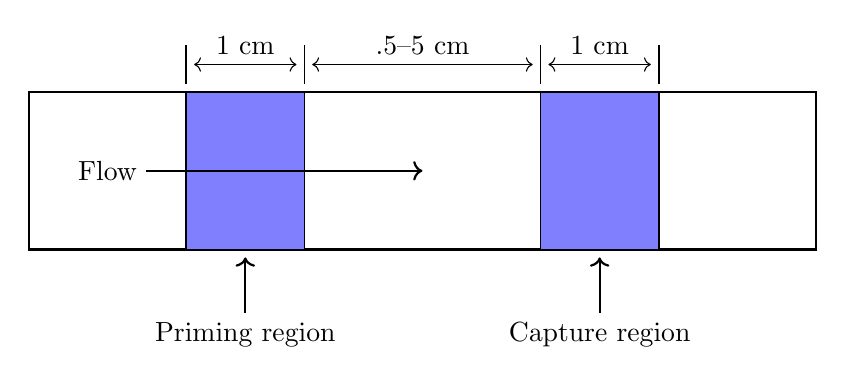
\begin{tikzpicture}
  \draw[thick] (-5, -1) rectangle (5, 1);
  \filldraw[semithick, fill=blue!50] (-3, -1) rectangle (-1.5, 1);
  \filldraw[semithick, fill=blue!50] (1.5, -1) rectangle (3, 1);
  \draw[thick, ->] (-4, 0) node[fill=white] {Flow} -- (0, 0);
  \draw[thick, ->] (-2.25, -1.8) node[below] {Priming region} -- ++(0, .7);
  \draw[thick, ->] (2.25, -1.8) node[below] {Capture region} -- ++(0,
  .7);
  \draw[semithick] (-3, 1.1) -- +(0, .5);
  \draw[semithick] (-1.5, 1.1) -- +(0, .5);
  \draw[semithick] (1.5, 1.1) -- +(0, .5);
  \draw[semithick] (3, 1.1) -- +(0, .5);
  \draw[<->] (-2.9, 1.35) -- node[midway, above] {1 cm} +(1.3, 0);
  \draw[<->] (1.6, 1.35) -- node[midway, above] {1 cm} +(1.3, 0);
  \draw[<->] (-1.4, 1.35) -- node[midway, above] {$.5$--$5$ cm}(1.4,
  1.35);
\end{tikzpicture}

%   \caption[Schematic of the microfluidic chambers]{Schematic of the
%     microfluidic chambers used in the priming experiments from the PPI
%     group. Blood is perfused from left to right over the priming and
%     capture regions. Either immobilized agonist or a nonreactive
%     control is printed in the priming and capture regions}
%   \label{fig:flow-chamber}
% \end{figure}

In previous research, the PPI group has found that all three
immobilized platelet agonists tested (vWF, collagen, and fibrinogen)
in the upstream region increased adhesion of platelets in the capture
region relative to a nonreactive control
\cite{Corum2012,Eichinger2016}. Recent work has shown similar results
when the upstream agonist printing was replaced by a stenotic region
with higher wall shear rates \cite{Rahman2020,Rahman2021}. In
addition, flow cytometry has revealed that platelets in blood which
has been perfused over surface-immobilized agonists express higher
concentrations of several different activation markers
\cite{Corum2012,Eichinger2016}.

In addition to the adhesion and flow cytometry experiments, the PPI
group is studying the effect of priming on the rolling behavior of
platelets over immobilized agonists. In this set of experiments, a
camera captures video of platelets rolling along the capture region,
and from this data they extract average platelet rolling velocities,
average step sizes, and pause times of rolling platelets. The step
size is defined to be the distance a platelet travels in the direction
of flow in between binding to the wall, and the pause time is defined
to be the length of time a platelet spends transiently attached to the
wall in between steps.

While flow cytometry is a useful tool to precisely measure quantities
of active receptors and other proteins, platelets must be incubated
with marker chemicals for 20 minutes before measurement, making the
measurements of platelet activation markers temporally imprecise. On
the other hand, the behavior of rolling platelets can be observed in
real time, but the relationship between rolling behavior and platelet
activation state is not clear. 

\section*{Methods (or Materials and Methods?)}

\subsection*{Experimental data and platelet trajectories}

The experimental materials and methods used to track platelets as they
roll along an agonist-coated surface are described in
\cite{Pumford2021}. This setup and data analysis is summarized briefly
below.

\subsubsection*{Flow chamber setup}

To mimic biologically flowing whole blood interactions with
immobilized proteins, specific agonists were printed onto amine-coated
slides in two regions: an upstream priming region, and a downstream
rolling region. Flow channels were then assembled and perfused with
fresh, whole blood labeled with fluorescent molecules at a wall shear
rate of 100 $s^{-1}$. Fluorescent microscope videos were taken in the
downstream rolling region using ImageJ acquisition software, and
analyzed using the MTrackJ plugin to manually track rolling platelets.

\subsubsection*{Platelet trajectory analysis}

A platelet trajectory is defined as the platelet's displacement in the
flow direction as a function of time. Trajectories were split into two
distinct states: pauses (when the platelet is stationary), and steps
(when the platelet is in motion). The time in which a platelet remains
stationary (within a single pause) is defined as the pause time, and
the distance each platelet traveled between pause events was defined
as the step size. Similarly, step \emph{times} are defined as the
times in between pause events where a platelet is in a step. Any
trajectories where the platelet did not pause were excluded from the
analysis. Steps and pauses which occurred at the beginning or end of a
trajectory were excluded from the step size and pause time data,
respectively.

Steps which occurred at the beginning and end of platelet trajectories
were significantly larger than steps which occurred between pause
events (supplementary material). Therefore, platelet trajectories were
``trimmed'' so that they began at the start of the first pause event,
and ended at the end of the last pause event.

% Put this at the end of the introduction?
% Trajectories for two sets of data were analyzed. One set of
% trajectories was generated by unprimed platelets. In these
% experiments, inert HSA (

\subsection*{Four-state platelet model}

In the model, platelets can exist in four possible states: unbound
($\stateUnbound$), fast-bound ($\stateBoundF$), slow-bound
($\stateBoundS$), and both fast- and slow-bound ($\stateBoundFS$) (see
Figure \ref{fig:primed-states}). Unbound platelets ($\stateUnbound$)
advect at a velocity $\jvVel$ in the fluid, and platelets in any of
the other states are bound to the wall and stationary. Unbound
platelets can bind through fast receptors at a constant rate
$\jvOnFast$ or through slow receptors at a constant rate
$\jvOnSlow$. A fast-bound platelet can bind through slow receptors at
the rate $\jvOnSlow$ to become a fast- and slow-bound platelet, or it
can unbind from the wall at the rate $\jvOffFast$.

Similar transitions can occur for slow-bound platelets and fast- and
slow-bound platelets. The rates $\jvOnFast$, $\jvOffFast$,
$\jvOnSlow$, and $\jvOffSlow$ are effective on and off rates for the
entire platelet, and \emph{not} on/off rates for individual
receptors. This model describes a jump-velocity process, where a
particle is transitioning randomly between discrete states, which each
move with a different deterministic motion. That is, the particle 
``jumps'' between different velocities depending on its random
transitions between states.

\begin{figure}
  \centering

  \schemestart
  $\stateUnbound$ \arrow(uu--vv){<=>[$\jvOnFast$][$\jvOffFast$]} $\stateBoundF$
  \arrow(@uu--ff){<=>[*{0}$\jvOnSlow$][*{0}$\jvOffSlow$]}[-90] $\stateBoundS$
  \arrow(--vf){<=>[$\jvOnFast$][$\jvOffFast$]} $\stateBoundFS$
  \arrow(@vv--@vf){<=>[*{0}$\jvOnSlow$][*{0}$\jvOffSlow$]}
  \schemestop

  \caption{A platelet can exist in four states: ($\stateUnbound$) unbound
    from the surface and advecting in the fluid, ($\stateBoundF$) bound
    through fast-bonds to the surface, ($\stateBoundS$) bound to slow-bonds
    to the surface, or ($\stateBoundFS$) bound through both fast and slow
    bonds. In all three bound states, the platelet is immobilized on
    the surface. Transitions that involve forming or breaking a fast
    bond with the surface occur at rates $\jvOnFast$ and $\jvOffFast$,
    respectively. Transitions that involve forming or breaking a slow
    bond with the surface occur at rates $\jvOnSlow$ and
    $\jvOffSlow$.}
  \label{fig:primed-states}
\end{figure}

\subsubsection*{Fokker-Planck equations}

The Fokker-Planck equations for these processes are given by the
following system of linear advection equations:
\begin{equation}
  \label{eq:fp-system}
  \Pder{}{t}
  \begin{pmatrix}
    p_{00} \\  p_{01} \\ p_{10} \\ p_{11}
  \end{pmatrix}
  =
  -\Pder{}{x}
  \begin{pmatrix}
    \jvVel p_{00} \\ 0 \\ 0 \\ 0
  \end{pmatrix}
  + 
  \begin{pmatrix}
    -(\jvOnFast + \jvOnSlow) & \jvOffFast & \jvOffSlow & 0 \\
    \jvOnFast & -(\jvOffFast + \jvOnSlow) & 0 & \jvOffSlow \\
    \jvOnSlow & 0 & -(\jvOnFast + \jvOffSlow) & \jvOffFast \\
    0 & \jvOnSlow & \jvOnFast & -(\jvOffFast + \jvOffSlow)
  \end{pmatrix}
  \begin{pmatrix}
    p_{00} \\ p_{01} \\ p_{10} \\ p_{11}
  \end{pmatrix}
\end{equation}
where $p_i = p_i(x, t \mid x_0, j, 0)$ is the probability the platelet
is in state $i$ and position $x$ at time $t$ given it was in position
$x_0$ and state $j$ at time $0$.

The Fokker-Planck equations can be used to find the probability
density function of the average velocity of a platelet traversing a
segment of length $L$. Assuming all platelets enter the interval
$[0, L]$ unbound, we take the initial condition of the PDE system
(\ref{eq:fp-system}) to be
$\vect{p}(x, 0) = (\delta(x), 0, 0, 0)^T$. The probability density
of the time it takes a platelet to cross the domain is
$\jvVel (p_{00}(L,t))$ (because the platelet is immobile in the other
3 states, it \emph{must} be in the $\stateUnbound$ state when it
leaves the domain). The average velocity associated with a crossing
time $t^*$ is just $v^* = L/t^*$, and the probability density function
of $v^*$ is given by $f(v^*) = Lv/(v^*)^2 p_U(L, L/v^*)$.

\subsubsection*{Fast-slow subsystems}

Biologically, platelet interaction with a surface in the bloodstream
is mediated by fast and slow bonds, which suggests there may be a fast
time scale in the Fokker-Planck system. There is also experimental
evidence for a fast time scale involved with platelet
rolling. Platelet velocities in between pause events were
significantly slower than velocities in steps at the beginning or end
of trajectories (supplementary material). These velocities in between
pauses were several times lower than the free-flowing velocity of a
platelet in a 100/s shear flow. One possible explanation of this
phenomenon is that there is fast binding and unbinding occurring on a
scale too fast to observe the individual events.

The relevant time scales to consider in the model are $T = L / v$ (the
time it takes an unbound platelet to cross the domain), and
$1 / \jvOnFast + \jvOffFast$ (the sum of the fast reaction
rates). Equation (\ref{eq:fp-system}) can be reduced under the
assumption that $1 / (T (\jvOnFast + \jvOffFast)) \ll 1$. The details
of the nondimensionalization and reduction are given in the
supplementary material, but they are summarized here.

The nondimensional variables $s$ and $y$ are defined so that $t = Ts$
and $x = Xy$. The displacement $x$ is scaled by the domain length, so
$X = L$, and $t$ is scaled so that
$X/T = \jvVel \implies T = L/\jvVel$. That is, $T$ is the shortest
possible crossing time of a platelet. Finally, the following
nondimensional parameters are defined:
$\epsilon_1 = 1/(T(\jvOnFast + \jvOffFast))$ and
$\epsilon_2 = 1/(T(\jvOnSlow + \jvOffSlow))$. After the
nondimensionalization, equation (\ref{eq:fp-system}) becomes
\begin{equation}
  \label{eq:nd-system}
  \Pder{\vect{q}}{s} = -\Pder{}{y}
  \begin{pmatrix}
    q_{00} \\ 0 \\ 0 \\ 0
  \end{pmatrix}
  + \left[\left(\frac{1}{\epsilon_1}\right) 
  \begin{pmatrix}
    - b & a & 0 & 0 \\
    b & - a & 0 & 0 \\
    0 & 0 & - b & a \\
    0 & 0 & b & - a
  \end{pmatrix} + \left(\frac{1}{\epsilon_2}\right)
  \begin{pmatrix}
    - d & 0 & c & 0 \\
    0 & - d & 0 & c \\
    d & 0 & - c & 0 \\
    0 & d & 0 & - c
  \end{pmatrix}\right]
  \vect{q},
\end{equation}
where $a = \jvOffFast/(\jvOffFast + \jvOnFast)$,
$b = \jvOnFast/(\jvOffFast + \jvOnFast)$,
$c = \jvOffSlow/(\jvOffSlow + \jvOnSlow)$, and
$d = \jvOnSlow/(\jvOffSlow + \jvOnSlow)$. In the nondimensional
system, the probability density function for the average velocity
across an inteval of unit length is $f(v^*) = ({v^*})^{-2} q_{00}
\left(1, 1/v^*\right)$.

Defining the first and second matrices from equation
(\ref{eq:nd-system}) as $A$ and $B$ respectively, equation
(\ref{eq:nd-system}) can be rewritten in the more compact form
\begin{equation}
  \label{eq:four-par-ad-fp}
  \Pder{\mathbf{q}}{s} = - \Pder{q_{U}}{y} \mathbf{e}_1 +
  \frac{1}{\epsilon_1} A \mathbf{q} + \frac{1}{\epsilon_2} B
  \mathbf{q}.
\end{equation}
The fast reactions are those captured in matrix $A$, so this matrix
defines the separation of the system into fast and slow
subsystems. The fast reaction matrix $A$ has two null eigenvalues,
because it has two linearly independent rows and two dependent
rows. The left null-vectors of $A$ define the projection onto the slow
manifold, and the orthogonal projection projects onto the fast
manifold, but the reaction diagram in Figure \ref{fig:primed-states}
makes the fast-slow separation clearer.

The fast reactions are represented by the two horizontal reaction
lines in Figure \ref{fig:primed-states}, and so the $\stateUnbound$
and $\stateBoundF$ states define one subsystem where the reaction
within that system are fast, and transitions into or out of that
system are slow, and $\stateBoundS$ and $\stateBoundFS$ define the
other such subsystem. Thus the following two slow variables can be
defined: $v_1 = q_{00} + q_{01}$ and $v_2 = q_{10} + q_{11}$.

These slow variables then evolve according to the following system of
equations:
\begin{align}
  \label{eq:v1-reduced}
  \Pder{v_1}{t} &= -a \Pder{v_1}{y} + \epsilon_1 a b \frac{\partial^2
                  v_1}{\partial y^2} - \frac{d}{\epsilon_2} v_1 +
                  \frac{c}{\epsilon_2} v_2 \\
  \label{eq:v2-reduced}
  \Pder{v_2}{t} &= \frac{d}{\epsilon_2} v_1 - \frac{c}{\epsilon_2} v_2.
\end{align}
So, the slow system evolves like its own jump-velocity process, except
that now the advecting quantity has a small diffusive component (as a
result of fast binding and unbinding) in addition to the advective
component. Additionally, while the platelet is in the
$\stateUnbound$--$\stateBoundF$ subsystem (that is, it is not bound
through a slow-bond to the surface), its position is described
by a two state jump-velocity process. A platelet in a step is assumed
to be in the $\stateUnbound$--$\stateBoundF$ subsystem, and a platelet
in a pause is assumed to be in the $\stateBoundS$--$\stateBoundFS$
subsystem. 

\subsubsection*{Distribution of velocities and estimates of fast
  parameters}

The average velocity of a platelet when it is in the $v_1$ subsystem
(i.e. when it is in a step) is used to estimate the fast binding and
unbinding parameters $\jvOnFast$ and $\jvOffFast$. With the reduced
equations (\ref{eq:v1-reduced}) and (\ref{eq:v2-reduced}), the
probability distribution of the average velocity $v^*$ of a platelet
in the $v_1$ subsystem has an analytic expression:
\begin{equation}
  \label{eq:avg-vel-pdf}
  f\left(v^*\right) = \sqrt{\frac{1}{4\pi \epsilon_1 a b
      \left(v^*\right)^3}} \left(a + \frac{v^* - a}{2}\right)
  \exp\left[\frac{-\left(v^* - a\right)^2}{4\epsilon_1 a b v^*}\right].
\end{equation}
Equation (\ref{eq:avg-vel-pdf}) is then used to find maximum
likelihood estimates (see \cite{Bain1992}) of $a$ and $\epsilon_1$
(and by extension, $\jvOnFast$ and $\jvOffFast$). The likelihood
function for $a$ and $\epsilon_1$ was maximized iteratively using
SciPy's \cite{Virtanen2020} \verb|minimize| function, which implements
the BFGS algorithm for unconstrained optimization
\cite{Nocedal2006}.

\subsubsection*{Escape rate and estimates of slow parameters}

Because the trajectories are ``trimmed,'' and only the portion of the
trajectory between the first and last pause is considered, then the
length of each platelet trajectory is different in general. To account
for this, it is assumed that there is some escape rate $\jvEscape$,
which represents the rate that platelets escape the rolling regime,
and re-enter the bulk flow. For convenience in the adiabatic
reduction, in the model platelets can escape at a constant rate
$\jvEscape$ when they are in either the unbound state $\stateUnbound$
or the fast-bound state $\stateBoundF$. This modification makes a
small change to equation (\ref{eq:v1-reduced}); there is an additional
$- \frac{\jvEscape}{T} v_1$ term in the equation.

With the added escape term, the number of pauses in each trajectory is
geometrically distributed. When a platelet is in a step, one can think
of the platelet's next state as a Bernoulli trial. One possibility is
the platelet pauses after the step, which occurs with probability
$\hat{a} = \frac{\jvOnSlow}{\jvOnSlow + \jvEscape}$. The other
possibility is the platelet escapes, and this occurs with probability
$1 - \hat{a} = \frac{\jvEscape}{\jvOnSlow + \jvEscape}$ (Figure
\ref{fig:unbd-plt-fates}). Therefore the number of binding events that
occur before the platelet escapes is geometrically distributed, and
the probability mass function for the number of binding events $n$ is
$p(n) = (1 - \hat{a}) \hat{a}^{n - 1}$, where $n \ge 1$. Thus the mean
number of pauses that occur before an escape can be used to find
$\hat{a}$:
\begin{equation}
  \label{eq:avg-dwell-num}
  \mu_\tn{dwell num.}  = (1 - \hat{a})\inv = (\jvOnSlow + \jvEscape) /
  \jvEscape.
\end{equation}

\begin{figure}
  \centering
  % \begin{tikzpicture}
  %   \node (step) {Step};
  %   \node (escape) [right=of step] {Escape};
  %   \draw[-Stealth] (step.east)
  %   --node[above]{$\frac{\jvEscape}{\jvTot}$} (escape.west); 
  %   %  {$\frac{e}{\jvTot}$}
  %   \draw[-Stealth] (step.north east)
  %   to[to path={
  %     .. controls +(60:1.5) and +(120:1.5) .. (\tikztotarget)
  %     \tikztonodes}
  %   ] node[above]{$\frac{\jvOnSlow}{\jvTot}$} (step.north west); 
  % \end{tikzpicture}
  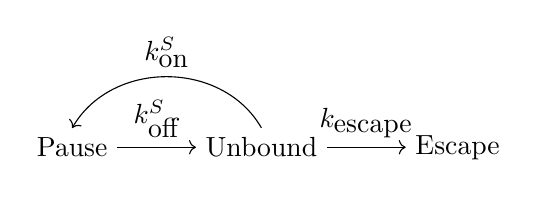
\begin{tikzpicture}
    \node (step)                    {Unbound};
    \node (escape)  [right=of step] {Escape};
    \node (pause)   [left=of step]  {Pause};
    \draw[->] (step.east) --node[above]{$\jvEscape$} (escape.west);
    \draw[->] (pause.east) --node[above]{$\jvOffSlow$} (step.west);
    \draw[->] (step.north)
    to[to path={
      .. controls +(120:1) and +(60:1) .. (\tikztotarget)
      \tikztonodes}
    ] node[above]{$\jvOnSlow$} (pause.north); 
  \end{tikzpicture}
  \caption{A platelet that is not bound to the surface has two
    possible fates: it can either re-bind with probability
    $\frac{\jvEscape}{\jvOnSlow + \jvEscape}$ (in which case it must
    unbind at some point again and return to the same state), or it
    can escape with probability
    $\frac{\jvOnSlow}{\jvOnSlow + \jvEscape}$.}
  \label{fig:unbd-plt-fates}
\end{figure}

\begin{figure}
  \centering
  \includegraphics[width=\textwidth]{fbg_num_dwells}
  \caption[Fit to dwell counts per trajectory]{Number of dwells per
    trajectory in experiments and predicted by a geometric
    distribution}
  \label{fig:ndwells}
\end{figure}

Another estimate is needed in order to uniquely find $\jvOnSlow$ and
$\jvEscape$. One way to think about the diagram in Figure
\ref{fig:unbd-plt-fates} is as a pair of competing Poisson
processes. The step process fires at a rate $\jvOnSlow$, and the
escape process fires at a rate $\jvEscape$. Then the fate of the
platelet is determined by whichever process fires first following the
end of a pause. Because the platelet's fate is determined by the
minimum of these two exponentially-distributed firing times, the step
times are also distributed exponentially, with rate
$\jvOnSlow + \jvEscape \equiv \jvTot$. Therefore an estimate of
$\jvTot$ can be found using the average step time:
\begin{equation}
  \mu_\tn{step time} = 1/\jvTot = 1/(\jvOnSlow + \jvEscape).
  \label{eq:average-step-time}
\end{equation}

Equations (\ref{eq:avg-dwell-num}) and (\ref{eq:average-step-time})
were simultaneously solved to get the following explicit expressions
for $\jvOnSlow$ and $\jvEscape$ in terms of $\mu_\tn{dwell num}$ and
$\mu_\tn{step time}$:
\begin{align}
  \label{eq:escape-estimate}
  \jvEscape &= \frac{1}{\mu_\tn{dwell num} \cdot \mu_\tn{step time}}
  \\
  \label{eq:slow-on-estimate}
  \jvOnSlow &= \frac{\mu_\tn{dwell num} - 1}{\mu_\tn{dwell num} \cdot
              \mu_\tn{step time}}.
\end{align}
Because the slow unbinding rate $\jvOffSlow$ is constant, the pause
times are exponentially distributed with mean $(\jvOffSlow)\inv$ and
$\jvOffSlow$ was estimated by taking the inverse of the mean pause
time:
\begin{equation}
  \label{eq:slow-off-estimate}
  \jvOffSlow = 1/\mu_\tn{pause}.
\end{equation}

% I haven't yet mapped states in the diagram to steps and pauses

% \begin{enumerate}[label=(\roman*)]
% \item Describe experimental setup and trajectory processing (exclude
%   the initial and final steps from analysis)
% \item Four-state jump-velocity model
%   \begin{itemize}
%   \item Define states and transitions (i.e. describe Figure 3.2)
%   \item State Fokker-Planck equations for the 4-state system, mention
%     the quasi-steady-state reduction, and give the two slow subsystems
%   \item Define the distribution of average velocities (within a step,
%     i.e. when the platelet is in either the U or V state), and mention
%     how this distribution is fit to data to estimate the fast on/off rates
%   \item Introduce escape term, and define the estimates of slow parameters
%   \item Describe simulation of trajectories
%   \end{itemize}
% \end{enumerate}

\section*{Results}

\subsection*{Estimates of fast on and off rates}

In order to estimate $\jvOnFast$ and $\jvOffFast$, experimental
trajectories were first processed by removing pauses and ``stacking''
the steps on top of each other. That is, for each original trajectory,
a modified trajectory was constructed which only consisted of the
platelet motion within steps. Then the average velocity for each of
these modified trajectories was calculated, and the average velocity
distribution in equation (\ref{eq:avg-vel-pdf}) was fit to these data
(Figure \ref{fig:fbg-whl-vel-fit}).

Means of average step velocities were not significantly different
($p = 0.81$) between experiments with ($9.83 \pm 1.11 \, \mu
\tn{m}/\tn{s}$) and without ($9.07 \pm 2.61 \, \mu \tn{m}/\tn{s}$)
priming. Therefore the model velocity distribution was fit to both
sets of data simultaneously. The estimates given after fitting were
$\jvOnFast = 61.0 / \tn{s}$ and $\jvOffFast = 8.14 / \tn{s}$.

% \begin{figure}
%   \centering
%   \includegraphics[width=\textwidth]{col_vel_fit}
%   \caption[Fits to average free velocity, collagen]{Comparison of the
%     average free velocity in four experimental conditions. The
%     two-state model was fit to all data simultaneously, and the fit
%     parameters for the fast reactions are $\jvOnFast = 14.82 / s$ and
%     $\jvOffFast = 2.98 / s$. The plot on the left shows a histogram of
%     average free velocities for 4 different experimental conditions,
%     and the distribution of average free velocities in the
%     jump-velocity model after fitting the fast binding and unbinding
%     parameters. The plot on the right compares the CDF from the model
%     fit with the empirical CDFs from the experimental data.}
%   \label{fig:col-vel-fit}
% \end{figure}

\begin{figure}
  \centering
  \includegraphics[width=\textwidth]{fbg_whl_vel_fit}
  \caption[Fits to average step velocity]{Comparison of the average
    step velocity in unprimed and primed experimental
    conditions. Equation (\ref{eq:avg-vel-pdf}) was fit to both sets
    of data simultaneously, and the fit parameters are
    $\jvOnFast = 61.0 / s$ and $\jvOffFast = 8.14$. The plot on the
    left shows a histogram of average step velocities of platelets
    with and without priming, and the distribution of average step
    velocities in the jump-velocity model after fitting the fast
    binding and unbinding parameters. The plot on the right compares
    the CDF from the model fit with the empirical CDFs from the
    experimental data.}
  \label{fig:fbg-whl-vel-fit}
\end{figure}

% These figures---and some later figures---use a three
% letter code as a shorthand for different experimental setups. The
% first two letters in the code give the chemical that is printed in the
% upstream priming region (the first letter) and the downstream rolling
% region (the second letter). In these codes, ``c'' stands for collagen,
% ``f'' stands for fibrinogen, and ``h'' stands for albumin, which is an
% inert material. The final letter in the code says whether the
% experiment was performed with whole blood (w) or platelet-rich plasma
% (p). Therefore the code ``ccw'' means an experiment with whole blood
% where collagen is printed in the upstream priming region and the
% downstream rolling region. The fast effective binding parameters
% predicted by each model fit are given in the captions below each
% figure.

% What about fitting to individual dwells? This might make it easier
% to bootstrap uncertainty estimates of the parameters. This would
% probably also be a more convincing analysis that the free velocities
% don't change between experiments than an ANOVA

\subsection*{Estimates of slow on and off rates}

Next, the slow parameters $\jvOnSlow$, $\jvOffSlow$, and $\jvEscape$
were estimated for experiments with and without priming using
equations (\ref{eq:escape-estimate})--(\ref{eq:slow-off-estimate}).
The results of these fits are shown in Table \ref{tab:par-est}. There
is not a significant difference ($p = 0.42$) between estimates of
$\jvOffSlow$ in the experiments with ($0.16 \pm 0.03 \tn{s}\inv$) and
without ($0.14 \pm 0.06 \tn{s}\inv$) priming. However, there is an
approximately 50-fold increase in $\jvOnSlow$ estimated from the
experiment with priming ($5.24 \pm 1.25 \tn{s}\inv$) relative to the
experiment without priming ($0.13 \pm 0.12 \tn{s}\inv$). This
difference is significant, with a $p$-value of $3.0 \times 10^{-11}$.

Curiously, the model also predicts a significant increase
($p = 8.0\times 10^{-5}$) in the escape rate in the experiment with
priming ($2.42 \pm 0.58 \tn{s}\inv$) over the experiment without
priming ($0.48 \pm 0.47 \tn{s}\inv$). One possible explanation for
this is that it is an artifact of the finite field of view in the
experiments. Having a fixed field of view could artificially increase
the estimate of the escape rate because the field of view limits the
number of dwells it is possible to observe in a single trajectory.

\begin{table}
  \centering
  \caption{Parameter estimates for the unprimed and primed experiments
    on fibrinogen}
  \begin{tabular}{rccc} \toprule
    & $\jvOnSlow$ & $\jvEscape$ & $\jvOffSlow$ \\ \midrule
    Primed & $5.24 \pm 1.25$ & $2.42 \pm 0.58$ & $0.16 \pm 0.03$ \\
    Unprimed & $0.13 \pm 0.12$ & $0.48 \pm 0.47$ & $0.14 \pm 0.06$ \\
    \bottomrule 
  \end{tabular}
  \label{tab:par-est}
\end{table}

To validate the estimates for $\jvOnSlow$ and $\jvEscape$ given in
Table \ref{tab:par-est}, the observed distribution of step times was
plotted with the distribution of step times generated from 128
stochastic simulations of the model using the parameters in Table
\ref{tab:par-est} (Figure \ref{fig:fbg-whl-step}). For experiments
with priming, the experimental and simulated distributions of step
sizes match well. In the experiments without priming, only 4 steps
occurred between dwells and it is more difficult to tell if the
experimental and simulated data match well, although it seems that the
simulations predict step times which are somewhat longer than what is
observed.

\begin{figure}
  \centering
  \includegraphics[width=\textwidth]{fbg_whl_step}
  \caption[Step times on fibrinogen]{Distribution of step times in
    experiments and in simulations of rolling on fibrinogen in whole
    blood.  The histogram in the left plot shows the distribution of
    step times in experiments. The plot on the right shows the
    empirical CDFs of the experimental data (solid lines) and the
    empirical CDFs of step sizes from stochastic simulations of the
    jump-velocity model (dash-dotted lines). The estimate for
    $\jvOnSlow$ from the hfw data (unprimed platelets) is
    $0.13 \pm 0.12 \tn{s}\inv$, and the estimate for $\jvOnSlow$ from the ffw
    data (primed platelets) is $5.24 \pm 1.25 \tn{s}\inv$.}
  \label{fig:fbg-whl-step}
\end{figure}

Figure \ref{fig:fbg-whl-pause} compares the pause times from
experiments on fibrinogen with 128 runs of the stochastic model with
the estimated parameters. The experimental and simulated distributions
of pause times track closely for experiments both with and without
priming. In the experiment with priming, the simulated pause times
slightly underestimate the prevalence of short pause times.

\begin{figure}
  \centering
  \includegraphics[width=\textwidth]{fbg_whl_pause}
  \caption[Pause times on fibrinogen]{Distribution of pause times in
    experiments and in simulations of rolling on fibrinogen. Each of
    the plots shows the same information as Figure \ref{fig:fbg-whl-step},
    but for pause times on fibrinogen. The estimates for $\jvOffSlow$
    are: hfw---$0.14 \pm 0.06 \tn{s}\inv$, ffw---$0.16 \pm 0.03 \tn{s}\inv$.}
  \label{fig:fbg-whl-pause}
\end{figure}

In order to test the hypothesis that the number of pauses per
trajectory is geometrically distributed, Figure \ref{fig:ndwells}
compares the observed distribution of the number of pauses with a
geometric distribution. The geometric distribution overestimates the
proportion of trajectories with a small number of pauses, but
otherwise there is good agreement between the two distributions.

\begin{figure}
  \centering
  \includegraphics[width=\textwidth]{fbg_num_dwells}
  \caption[Fit to pause counts per trajectory]{Number of pauses per
    trajectory in experiments (density histogram) and predicted by a
    geometric distribution (stars).}
  \label{fig:ndwells}
\end{figure}

Finally, to illustrate the types of trajectories predicted by the
jump-velocity model, Figure \ref{fig:fbg-whl-traj-sim} plots
experimental trajectories of primed and unprimed platelets on
fibrinogen, and simulated trajectories with the parameters given in
Table \ref{tab:par-est}. As was shown in Figure \ref{fig:ndwells}, for
both experiments some of the simulated trajectories have more dwells
than any of the experimental trajectories. However apart from this,
the simulated trajectories are qualitatively similar to experimental
trajectories. 

\begin{figure}
  \centering
  \includegraphics[width=\textwidth]{fbg_whl_traj_sim}
  \caption[Platelet trajectories on fibrinogen]{Experimental and
    simulated platelet trajectories on fibrinogen in whole blood. Blue
    curves show trajectories from unprimed platelets, and red curves
    show trajectories from primed platelets. The plot on the left
    shows trajectories from experimental data. The plot on the right
    shows a set of simulated trajectories from the stochastic
    jump-velocity model, with parameters fit to the experimental data
    as shown above.}
  \label{fig:fbg-whl-traj-sim}
\end{figure}

% \begin{enumerate}[label=(\roman*)]
% \item Estimates of fast on and off rates (Figure 3.11): these rates do
%   not change with priming, and the estimated rates are significantly
%   faster than the estimates for the slow rates.
% \item Estimates of slow on/off and escape rates (Figures 3.13--3.15
%   and Table 3.2): the off rate doesn't change with priming, but the on
%   rate increases by a factor of $\sim 50$.
% \item Comparison of experimental and simulated platelet trajectories
%   (Figure 3.16). We can also potentially include trajectories from 3D
%   simulations. 
% \end{enumerate}

\section*{Discussion}

In the modeling framework laid out above, the only spatial dimension
considered is the axis in the direction of flow. Platelets are assumed
to be infinitesimal particles immersed in the flow which bind and
unbind with a single effective rate, and only move at two velocities:
a constant free-flowing velocity, and zero velocity. Any interactions
with other cells in the blood are ignored. Furthermore, all platelets
are assumed to have the same binding and unbinding rates. All of these
assumptions greatly simplify the description of platelet rolling and
binding with an agonist-coated surface, but allow for precise
estimation of model parameters.

Parameters mediating the fast binding of platelets to the surface were
estimated by fitting the platelet velocities in between pauses to a
velocity distribution generated by a quasi-steady-state reduction of
the four-state Fokker-Planck equation. On immobilized fibrinogen, the
fast bonds are likely mediated by GP1b bonds with vWF adhered to the
immobilized fibrinogen (source). Therefore the estimates of
$\jvOnFast$ and $\jvOffFast$ above provide estimates of platelet
association and dissociation with an agonist-coated surface medated by
GP1b-vWF bonds. The estimates for the fast on and off rates did not
change with priming.

Next, step times, pause times, and number of dwells per trajectory
were used to estimate parameters for binding mediated by slow
receptor-ligand binding. On fibrinogen, unprimed platelets had a small
binding rate---around $0.1 \tn{s}\inv$, but after activation the
binding rate increased by a factor of nearly 50 (Table
\ref{tab:par-est}). The slow unbinding rate remained around
$0.1 \tn{s}\inv$ for both the unprimed and primed experiments. The
observation that the binding rate of \ITA{IIb}\ITB{3}-fibrinogen
increased with integrin activation, while the unbinding rate remained
unchanged, is consistent with the observations of \cite{Litvinov2012}.


% \section*{Conclusion}

% \section*{Author Contributions}

% Author1 designed the research. Author2 carried out all simulations, analyzed the data. Author1 and Author2 wrote the article. 

% \section*{Acknowledgments}

% We thank G. Harrison, B. Harper, and J. Doe for their help.

% Uncomment if using bibtex (default)
\bibliography{jv-paper}

% Uncomment if using biblatex
% \printbibliography

% \section*{Supplementary Material}

% An online supplement to this article can be found by visiting BJ Online at \url{http://www.biophysj.org}.

\end{document}







